\chapter{Seifert-Vankampen Theorem}

\begin{theorem}
    Let $K= K_1 \cup K_2$ be topological spaces with
    \begin{itemize}
        \item $K_1,K_2$ path-connected open in $K$
        \item $K_1 \cap K_2$ path-connected
    \end{itemize}
    Take $b \in K_1 \cap K_2$. Suppose
    \begin{align*}
        &\Pi_1(K_1,b) \cong \langle X_1 \mid R_1 \rangle\\
        &\Pi_1(K_2,b) \cong \langle X_2 \mid R_2 \rangle
    \end{align*}
    with $i_1: K_1 \cap K_2 \rightarrow K_1$ and $i_2: K_1 \cap K_2 \rightarrow K_2$ inclusion maps. Then
    \begin{align*}
        \Pi_1 (K,b) &\cong \langle X_1,X_2 \mid R_1,R_2, (i_1)_*(\alpha) = (i_2)_* (\alpha)\; \forall \alpha \in \Pi_1 (K_1 \cap K_2, b) \rangle\\
        &\cong \Pi_1(K_1,b) *_{\Pi_1 (K_1 \cap K_2,b)} \Pi_1 (K_2,b)
    \end{align*}
    here $*$ is called the \textit{Amalgamation Product}.
\end{theorem}

\noindent\textbf{Example:} 


\begin{enumerate}
    \item \begin{center}
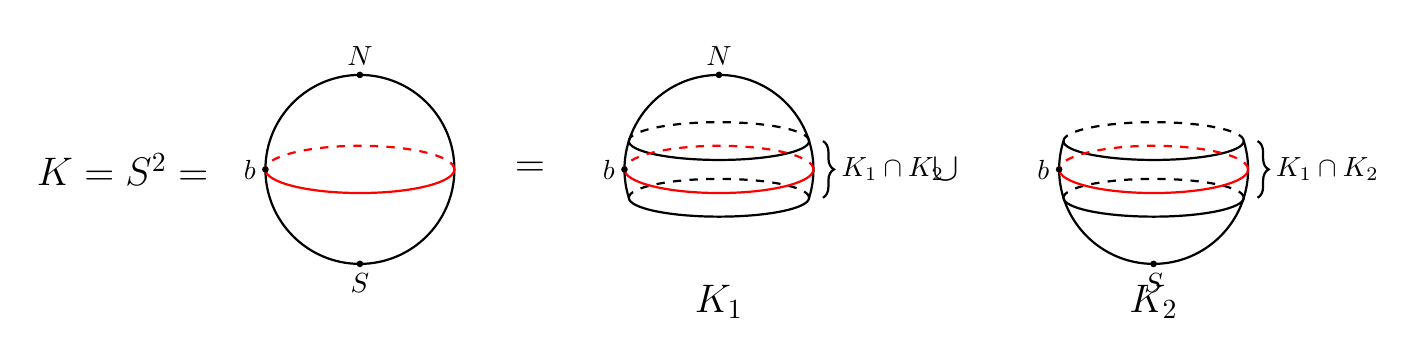
\begin{tikzpicture}[x=1.2cm, y=1.2cm, >=stealth]
    
    
    \node[left] at (-1.5, 0) {\Large $K = \mathbb{S}^2 =$};
    
    \begin{scope}[shift={(0,0)}]
        \draw[thick] (0,0) circle (1);
        
        
        \draw[thick, red] (-1,0) arc (180:360:1 and 0.25);
        \draw[thick, red, dashed] (1,0) arc (0:180:1 and 0.25);
        
        
        \fill (0,1) circle (1.2pt) node[above] {$N$};
        \fill (0,-1) circle (1.2pt) node[below] {$S$};
        \fill (-1,0) circle (1.2pt) node[left] {$b$};
    \end{scope}
    
    \node at (1.8, 0) {\Large $=$};
    
    
    \begin{scope}[shift={(3.8,0)}]
        
        \begin{scope}
            \clip (-1.5, -0.3) rectangle (1.5, 1.5);
            \draw[thick] (0,0) circle (1);
        \end{scope}
        
        
        \draw[thick] (-0.954, 0.3) arc (180:360:0.954 and 0.2);
        \draw[dashed, thick] (0.954, 0.3) arc (0:180:0.954 and 0.2);
        
        
        \draw[thick] (-0.954, -0.3) arc (180:360:0.954 and 0.2);
        \draw[dashed, thick] (0.954, -0.3) arc (0:180:0.954 and 0.2);
        
        
        \draw[thick, red] (-1, 0) arc (180:360:1 and 0.25);
        \draw[dashed, thick, red] (1, 0) arc (0:180:1 and 0.25);
        
        
        \fill (0,1) circle (1.2pt) node[above] {$N$};
        \fill (-1,0) circle (1.2pt) node[left] {$b$};
        \node at (0, -1.4) {\Large $K_1$};
        
        
        \draw[decorate,decoration={brace,amplitude=4pt},thick] (1.1, 0.3) -- (1.1, -0.3) node[midway,right,xshift=3pt] {$K_1 \cap K_2$};
    \end{scope}

    \node at (6.2, 0) {\Large $\cup$};

    
    \begin{scope}[shift={(8.4,0)}]
        
        \begin{scope}
            \clip (-1.5, -1.5) rectangle (1.5, 0.3);
            \draw[thick] (0,0) circle (1);
        \end{scope}
        
        
        \draw[thick] (-0.954, 0.3) arc (180:360:0.954 and 0.2);
        \draw[dashed, thick] (0.954, 0.3) arc (0:180:0.954 and 0.2);
        
        
        \draw[thick] (-0.954, -0.3) arc (180:360:0.954 and 0.2);
        \draw[dashed, thick] (0.954, -0.3) arc (0:180:0.954 and 0.2);
        
        
        \draw[thick, red] (-1, 0) arc (180:360:1 and 0.25);
        \draw[dashed, thick, red] (1, 0) arc (0:180:1 and 0.25);
        
        
        \fill (0,-1) circle (1.2pt) node[below] {$S$};
        \fill (-1,0) circle (1.2pt) node[left] {$b$};
        \node at (0, -1.4) {\Large $K_2$};
        
        
        \draw[decorate,decoration={brace,amplitude=4pt},thick] (1.1, 0.3) -- (1.1, -0.3) node[midway,right,xshift=3pt] {$K_1 \cap K_2$};
    \end{scope}

\end{tikzpicture}
\end{center}



\begin{align*}
\text{Then} \qquad K_1 \simeq \{N\} &\implies \pi_1(K_1, b) \cong \langle e \rangle = \langle \alpha \mid \alpha \rangle \\[4pt]
K_2 \simeq \{S\} &\implies \pi_1(K_2, b) \cong \langle e \rangle = \langle \beta \mid \beta \rangle \\[4pt]
K_1 \cap K_2 \simeq \mathbb{S}^1 &\implies \pi_1(K_1 \cap K_2, b) \cong \mathbb{Z} = \langle \gamma \mid \emptyset \rangle
\end{align*}

\vspace{0.2cm}
\noindent Hence, \quad $(i_1)_* : \pi_1(K_1 \cap K_2, b) \longrightarrow \pi_1(K_1, b)$ \quad and \quad $(i_2)_* : \pi_1(K_1 \cap K_2, b) \longrightarrow \pi_1(K_2, b)$

\vspace{0.2cm}
\noindent \hspace{3.8cm} $\gamma \longmapsto e$ \hspace{5.2cm} $\gamma \longmapsto e$

\vspace{0.5cm}
\noindent Then, apply Seifert-Vankampen Th'm,
\begin{align*}
\pi_1(K, b) &= \langle \alpha, \beta \mid \alpha, \beta, (i_1)_*(\gamma^n) = (i_2)_*(\gamma^n) \quad \forall n \in \mathbb{Z} \rangle \\[6pt]
&= \langle \alpha, \beta \mid \alpha, \beta, e=e \rangle = \langle e \rangle
\end{align*}

    

    \vspace{5cm}
    \item \begin{center}
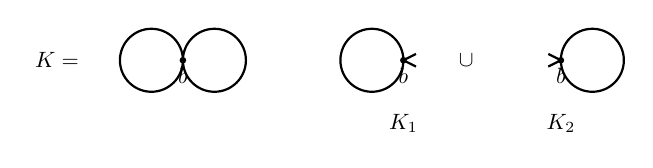
\begin{tikzpicture}[scale=0.8, every node/.style={transform shape}]
    
    
    \node at (-1.5, 0.5) {$K = $};
    \draw[thick] (0,0.5) circle (0.5);
    \draw[thick] (1,0.5) circle (0.5);
    \fill (0.5,0.5) circle (1.5pt) node[below] {$b$};
    
    

    
    \begin{scope}[shift={(3.5, 0)}]
        \draw[thick] (0,0.5) circle (0.5);
        \draw[thick] (0.5,0.5) -- (0.7, 0.6);
        \draw[thick] (0.5,0.5) -- (0.7, 0.4);
        \fill (0.5,0.5) circle (1.5pt) node[below] {$b$};
        
        \node at (0.5, -0.5) {$K_1$};
    \end{scope}

    \node at (5, 0.5) {$\cup$};

   
    \begin{scope}[shift={(6, 0)}]
        \draw[thick] (1,0.5) circle (0.5);
        \draw[thick] (0.5,0.5) -- (0.3, 0.6);
        \draw[thick] (0.5,0.5) -- (0.3, 0.4);
        \fill (0.5,0.5) circle (1.5pt) node[below] {$b$};
        
        \node at (0.5, -0.5) {$K_2$};
    \end{scope}
\end{tikzpicture}
\end{center}

\vspace{1em}
\noindent Then we have \quad $K_1 \simeq S^1 \implies \pi_1(K_1, b) \cong \langle \alpha \mid \emptyset \rangle$ \\[0.5em]
\phantom{Then we have \quad} $K_2 \simeq S^1 \implies \pi_1(K_2, b) \cong \langle \beta \mid \emptyset \rangle$ \\[0.5em]
\phantom{Then we have \quad} $K_1 \cap K_2 \simeq \{b\} \implies \pi_1(K_1 \cap K_2, b) \cong \langle e \rangle$

\vspace{1em}
\noindent Hence, $(i_1)_* : \alpha \mapsto e$ and $(i_2)_* : \beta \mapsto e$. Then by S-V Thm,
\[ \pi_1(K, b) \cong \langle \alpha, \beta \mid e = e \rangle \cong \langle \alpha, \beta \mid \emptyset \rangle \cong \mathbb{Z} * \mathbb{Z}. \]

\vspace{1em}
\noindent Then by induction, if $\Gamma$ is shown as figure 9.1,
\begin{figure}[htbp]
    \centering
    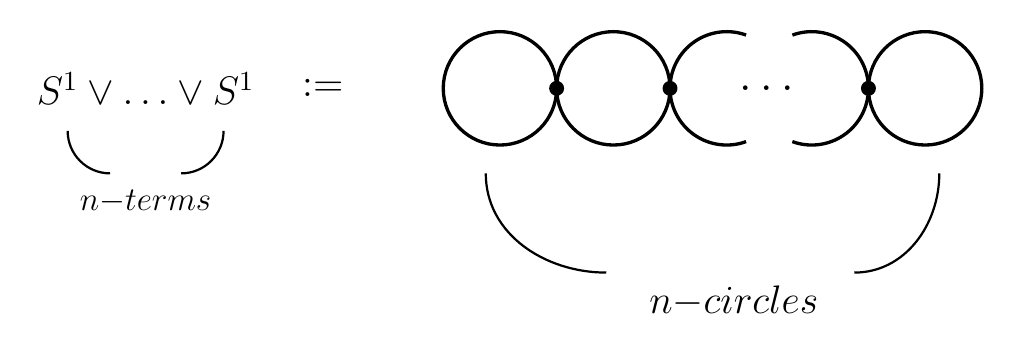
\begin{tikzpicture}[scale=0.9, very thick]
        
        
        \node at (-4, 0) {\Large $\mathbb{S}^1 \vee \dots \vee \mathbb{S}^1$};
        
        
        \draw[thick] (-5.1, -0.6) to[out=-90, in=180] (-4.5, -1.2);
        \draw[thick] (-2.9, -0.6) to[out=-90, in=0] (-3.5, -1.2);
        
        
        \node at (-4, -1.6) {\large $n\text{-terms}$};

        
        \node at (-1.5, 0) {\Large $:=$};

        
        \def\R{0.8}
        
        
        \draw (1, 0) circle (\R);
        \fill (1+\R, 0) circle (3pt);
        
        
        \draw (1+2*\R, 0) circle (\R);
        \fill (1+3*\R, 0) circle (3pt);
        
        
        \draw (1+3*\R, 0) arc (180:70:\R);
        \draw (1+3*\R, 0) arc (180:290:\R);
        
        
        \node at (1+4.7*\R, 0) {\LARGE $\dots$};
        
        
        \draw (1+6.5*\R, 0) arc (0:110:\R);
        \draw (1+6.5*\R, 0) arc (0:-110:\R);
        \fill (1+6.5*\R, 0) circle (3pt);
        
        
        \draw (1+7.5*\R, 0) circle (\R);

        
        \draw[thick] (0.8, -1.2) to[out=-90, in=180] (2.5, -2.6);
        \draw[thick] (1+7.5*\R + 0.2, -1.2) to[out=-90, in=0] (6.0, -2.6);
        
        
        \node at (4.3, -3.0) {\Large $n\text{-circles}$};

    \end{tikzpicture}
    \caption{Wedge sum of $n$ circles}
    \end{figure}
    then we have:
\[ \pi_1(\Gamma, b) \cong \underbrace{\mathbb{Z} * \cdots * \mathbb{Z}}_{n\text{-tuples}} \]

    \item $K= \mathbb{T}^2$
    

% 定义 TikZ 样式方便复用
\tikzset{
    dir_arrow/.style={postaction={decorate, decoration={markings, mark=at position 0.6 with {\arrow{Stealth}}}}},
    double_dir_arrow/.style={postaction={decorate, decoration={markings, mark=at position 0.6 with {\arrow{Stealth[sep=1pt]Stealth}}}}},
    dashed_box/.style={draw, dashed, minimum size=0.8cm},
}

\begin{center}
\begin{tikzpicture}[x=1.5cm, y=1.5cm]

% --- 第一行: K = K1 U K2 ---
% K 的正方形
\begin{scope}[shift={(0,0)}]
    \node at (-0.6, 0.5) {$K =$};
    \draw[thick, dir_arrow] (0,0) -- (1,0) node[below, midway] {$\alpha$};
    \draw[thick, double_dir_arrow] (1,0) -- (1,1) node[right, midway] {$\beta$};
    \draw[thick, dir_arrow] (0,1) -- (1,1) node[above, midway] {$\alpha$};
    \draw[thick, double_dir_arrow] (0,0) -- (0,1) node[left, midway] {$\beta$};
\end{scope}

\node at (1.5, 0.5) {\Large $=$};

% K1 的正方形（带孔）
\begin{scope}[shift={(2,0)}]
    \draw[thick, dir_arrow] (0,0) -- (1,0) node[below, midway] {$\alpha$};
    \draw[thick, double_dir_arrow] (1,0) -- (1,1) node[right, midway] {$\beta$};
    \draw[thick, dir_arrow] (0,1) -- (1,1) node[above, midway] {$\alpha$};
    \draw[thick, double_dir_arrow] (0,0) -- (0,1) node[left, midway] {$\beta$};
    \draw[dashed] (0.3, 0.3) rectangle (0.7, 0.7);
    \node at (0.5, -0.4) {$K_1$};
\end{scope}

\node at (3.5, 0.5) {\Large $\cup$};

% K2 的部分
\begin{scope}[shift={(4.2,0)}]
    \draw[dashed] (0.2, 0.3) rectangle (0.6, 0.7);
    \node at (0.4, -0.4) {$K_2$};
\end{scope}

% --- 第二行: 文字说明 ---
\node[anchor=west] at (-0.8, -1.2) {where \quad $K_1 \cap K_2 = \quad $};
\begin{scope}[shift={(1, -1.5)}]
    \draw[dashed] (0,0) rectangle (0.8, 0.8);
    \draw[dashed] (0.25, 0.25) rectangle (0.55, 0.55);
    \node at (1.3, 0.4) {$\simeq S^1$};
\end{scope}

% --- 第三行: 基本群同构 ---
\node[anchor=west] at (-1.2, -2.5) {$\Rightarrow \quad \pi_1(K_1) \cong \langle \alpha, \beta \rangle \quad , \quad \pi_1(K_2) \cong \langle e \rangle \quad , \quad \pi_1(K_1 \cap K_2) \cong \langle \gamma \rangle$.};

% --- 第四行: 包含映射 ---
% K1 cap K2 的圆圈图
\begin{scope}[shift={(-0.5, -4.5)}]
    \draw[dashed] (0,0) rectangle (1,1);
    \draw[dashed] (0.3, 0.3) rectangle (0.7, 0.7);
    \draw[thick, dir_arrow] (0.5, 0.5) circle (0.4);
    \node at (0.85, 0.25) {$\gamma$};
    \node at (0.5, -0.4) {$K_1 \cap K_2$};
\end{scope}

\draw[->] (1, -4) -- (1.8, -4) node[midway, above] {$i_1$};
\draw (1.1, -3.9) arc (120:240:0.15); % Subset notation curve

% K1 的圆圈映射图
\begin{scope}[shift={(2.5, -5)}]
    \draw[thick, dir_arrow] (0,0) -- (2,0) node[below, midway] {$\alpha$};
    \draw[thick, double_dir_arrow] (2,0) -- (2,2) node[right, midway] {$\beta$};
    \draw[thick, dir_arrow] (0,2) -- (2,2) node[above, midway] {$\alpha$};
    \draw[thick, double_dir_arrow] (0,0) -- (0,2) node[left, midway] {$\beta$};
    \draw[dashed] (0.5, 0.5) rectangle (1.5, 1.5);
    \draw[dashed] (0.8, 0.8) rectangle (1.2, 1.2);
    \draw[thick, dir_arrow] (1, 1) circle (0.7);
    \node at (1.6, 0.5) {$\gamma$};
    \node at (1, -0.4) {$K_1$};
\end{scope}

% 最终关系式
\node[anchor=west] at (5, -4) {\Large $\Rightarrow \quad i_{1*}(\gamma) = \alpha \beta \alpha^{-1} \beta^{-1}$};

\end{tikzpicture}
\end{center}

    It's easy to get $i_{2*} (\gamma) =e$. Then applying SVK,
    \begin{align*}
        \Pi_1 (\mathbb{T}^2) &\cong \langle \alpha,\beta \mid i_{1*} (\gamma) = i_{2*} (\gamma) \rangle
        \\&= \langle \alpha ,\beta \mid \alpha \beta \alpha^{-1} \beta^{-1} =e \rangle \cong \mathbb{Z} \oplus \mathbb{Z}
    \end{align*}

    \item $$\Pi_1 (\mathbb{T}^2 \# \mathbb{T}^2) \cong \Pi_1(\mathbb{T}^2) *_{\Pi_1(\mathbb{S}^1)} \Pi_1(\mathbb{T}^2) \cong \langle \alpha_1,\beta_1,\alpha_2,\beta_2 \mid [\alpha_1,\beta_1] [\alpha_2,\beta_2] =e \rangle$$

    \item $$\Pi_1(S_g) := \Pi_1(\#_{i=1}^g \mathbb{T}^2) \cong \langle \alpha_1,\beta_1 , \cdots ,\alpha_g,\beta_g \mid \Pi_{i=1}^g [\alpha_i ,\beta_i] =e \rangle$$
\end{enumerate}

\begin{proposition}
    Let $X,Y$ be two topological spaces with basepoints $x_0 \in X,y_0\in Y$. Then
    $$\Pi_1 (X\times Y, (x_0,y_0)) \cong \Pi_1(X,x_0) \times \Pi_1(Y,y_0)$$
\end{proposition}

\begin{proposition}
    Suppose $X,Y$ are of dimension $>2$. Then
    $$\Pi_1(X \# Y) \cong \Pi_1(X) * \Pi_1(Y)$$
\end{proposition}

\begin{proof}
    Since $\Pi_1 (\mathbb{S}^{n(\geq 2)}) \cong \langle e \rangle$, then
    $$\Pi_1(X \# Y) \cong \Pi_1(X) *_{\Pi_1 (\mathbb{S}^{n(\geq 2)})} \Pi_1(Y) \cong \Pi_1(X) *_{\{e\}} \Pi_1(Y) \cong \Pi_1(X) * \Pi_1(Y)$$
\end{proof}

\begin{proposition}
    Every closed (compact without boundary) orientable surface is given by $S_g$ for some $g \geq 0$.
\end{proposition}

\begin{definition}{Amalgamated Product}\\
Let $\{ H_{ij} \}_{(i,j)}$ be a symmetric collection of groups where we have a collection of homomorphisms
$$\{ \varphi_{ij} : H_{ij} \to G_i\}$$
The \textit{amalgamated product} of $\{G_i\}$ over $\{H_{ij} \}$ is defined as
$$*_{H_{ij}} G_i := *G_i / \langle \varphi_{ij} (\alpha) \varphi_{ji} (\alpha)^{-1} \mid \alpha \in H_{ij} \rangle$$
Here $\langle \varphi_{ij} (\alpha) \varphi_{ji} (\alpha)^{-1} \mid \alpha \in H_{ij} \rangle$ is cormal closure of set given by $\varphi_{ij} (\alpha) = \varphi_{ji} (\alpha)$, $\alpha \in H_{ij}$, for any $(i,j) \in J \times J$ in $*G_i$.

In presentation,
$$*_{H_{ij}} G_i = \langle \bigsqcup S_i \mid (\bigcup R_i) \cup (\{ \varphi_{ij} (\alpha) \varphi_{ji} (\alpha)^{-1} \mid \alpha \in H_{ij} \}) \rangle$$
\end{definition}

\noindent\textbf{Example:} $$F_2 *_\mathbb{Z} F_2 \cong F_3$$
This is by taking isomorphic copy of $\mathbb{Z}$ in $F_2$, i.e.:
$$\langle a,b,c,d \mid a=b \rangle \cong F_3$$

\begin{definition}{HNN-Extension}\\
Suppose $H,F \leq G$ are two isomorphic subgroups of $G$ given by $\varphi$ isomorphism. Let $\lambda \in F$. Then
$$\langle G,\lambda \mid \lambda^{-1} \alpha \lambda = \varphi (\alpha), \alpha \in H \rangle = G * \langle \lambda \rangle / \langle \lambda^{-1} \alpha \lambda \varphi(\alpha)^{-1} \mid \alpha \in H \rangle$$
\end{definition}

\noindent\textbf{Example:} Bamlog-Solitan Group:
$$BS(n,m) = \langle \alpha, \lambda \mid \lambda ^{-1} \alpha^n \lambda = \alpha^m \rangle \Rightarrow  BS(1,-1) = \Pi_1(Klein\;Bottle)$$

\begin{theorem}{Van-Kampen Theorem}\\
Suppose $X= \bigcup X_\alpha$ collection of open path-connected sets $X_\alpha$ with basepoint $x_0 \in X_\alpha$ $\forall \alpha$. If $X_\alpha \cap X_\beta$ are path-connected, then there is a unique surjective homomorphism
$$\Phi : *\Pi_1(X_\alpha) \to \Pi_1(X)$$
If in addition $X_\alpha \cap X_\beta \cap X_\gamma$ are path-connected, then $\ker \Phi$ is normal subgroup $N$ generated by
$$\langle i_{\alpha \beta*} (\omega) i_{\beta \alpha*}(\omega)^{-1} \rangle =N$$
i.e.: $\Pi_1(X) \cong *\Pi_1(X_\alpha)/N$
\end{theorem}

\begin{proof}
    First we show $\Phi$ is surjective. Given a loop $f: I \to X$ at the basepoint $x_0$, we may choose as in the proof of Proposition 1.5 a partition $0 = s_0 < s_1 < \cdots < s_m = 1$ so that each subinterval $[s_{i-1}, s_i]$ is mapped by $f$ to a single $A_\alpha$, which we denote $A_i$. Let $f_i$ be the path $f|_{[s_{i-1}, s_i]}$, so $f$ is the composition $f_1 \cdots f_m$. Since $A_i \cap A_{i+1}$ is path-connected, we may choose a path $g_i$ in $A_i \cap A_{i+1}$ from $x_0$ to the point $f(s_i) \in A_i \cap A_{i+1}$. Inserting $\bar{g}_i \cdot g_i$ into $f$ at $s_i$ for each $i$ then yields a loop
\[
(f_1 \cdot \bar{g}_1) \cdot (g_1 \cdot f_2 \cdot \bar{g}_2) \cdot (g_2 \cdot f_3 \cdot \bar{g}_3) \cdots (g_{m-1} \cdot f_m)
\]
homotopic to $f$. This loop is a composition of loops each lying in a single $A_i$, so $[f]$ is in the image of $\Phi$, and $\Phi$ is surjective.

\begin{center}
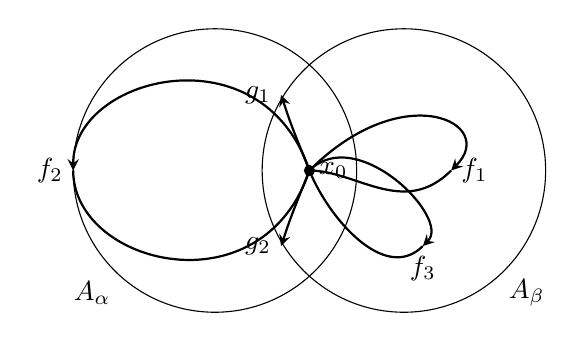
\begin{tikzpicture}[>=stealth, scale=1.2]
    % Draw two overlapping circles
    \draw (0,0) circle (1.5cm);
    \draw (2,0) circle (1.5cm);
    
    % Labels for sets
    \node at (-1.3,-1.3) {$A_\alpha$};
    \node at (3.3,-1.3) {$A_\beta$};
    
    % Basepoint x0
    \filldraw (1,0) circle (1.5pt) node[right] {$x_0$};
    
    % Path f1, f2, f3 etc.
    \draw[thick, ->] (1,0) .. controls (2,1) and (3,0.5) .. (2.5,0) node[right] {$f_1$};
    \draw[thick] (2.5,0) .. controls (2,-0.5) and (1.5,0) .. (1,0);
    
    \draw[thick, ->] (1,0) .. controls (0.5,1.5) and (-1.5,1) .. (-1.5,0) node[left] {$f_2$};
    \draw[thick] (-1.5,0) .. controls (-1.5,-1) and (0.5,-1.5) .. (1,0);
    
    \draw[thick, ->] (1,0) .. controls (1.5,0.5) and (2.5, -0.5) .. (2.2,-0.8) node[below] {$f_3$};
    \draw[thick] (2.2,-0.8) .. controls (1.8,-1.2) and (1.2,-0.5) .. (1,0);

    % Paths g1, g2
    \draw[thick, ->] (1,0) .. controls (0.8,0.5) .. (0.7,0.8) node[left] {$g_1$};
    \draw[thick, ->] (1,0) .. controls (0.8,-0.5) .. (0.7,-0.8) node[left] {$g_2$};
\end{tikzpicture}
\end{center}

The harder part of the proof is to show that the kernel of $\Phi$ is $N$. Suppose we are given a reduced word $w = w_1 \cdots w_k$ in $*_\alpha \pi_1(A_\alpha)$ such that $\Phi(w)$ is trivial. If we can show that $w$ has trivial image in $*_\alpha \pi_1(A_\alpha)/N$, then this will imply that the kernel of $\Phi$ is contained in $N$. The opposite inclusion has already been noted, so this will finish the proof.

Corresponding to the word $w = w_1 \cdots w_k$ there is a product $f = f_1 \cdots f_k$ of loops $f_i$ lying in $A_\alpha$'s. Since $\Phi(w)$ is trivial, there is a map $F: I \times I \to X$ defining a homotopy from $f$ to the constant loop. There exist partitions $0 = s_0 < s_1 < \cdots < s_m = 1$ and $0 = t_0 < t_1 < \cdots < t_n = 1$ such that each rectangle $R_{ij} = [s_{i-1}, s_i] \times [t_{j-1}, t_j]$ is mapped by $F$ into a single $A_\alpha$, which we label $A_{ij}$. These partitions may be obtained by covering $I \times I$ by finitely many rectangles $[a,b] \times [c,d]$ each mapping to a single $A_\alpha$, using a compactness argument, then partitioning $I \times I$ by the union of all the horizontal and vertical lines containing edges of these rectangles. We may assume the $s_i$-partition subdivides the partition decomposing $f$ as $f_1 \cdots f_k$. Since $F$ maps a neighborhood of $R_{ij}$ to $A_{ij}$, we may perturb the vertical sides of the rectangles $R_{ij}$ so that each point of $I \times I$ lies in at most three $R_{ij}$'s. We can do this perturbation just on the rectangles $R_{ij}$ with $j > 1$, leaving the rectangles $R_{i1}$ in the bottom row unchanged.

Let $f_{ij}$ be the loop obtained by restricting $F$ to the path in $I \times I$ which goes in linear segments from $(0, t_j)$ to the upper right corner of $R_{ij}$, then to the lower right corner of $R_{ij}$, then to $(1, t_{j-1})$.

\begin{center}
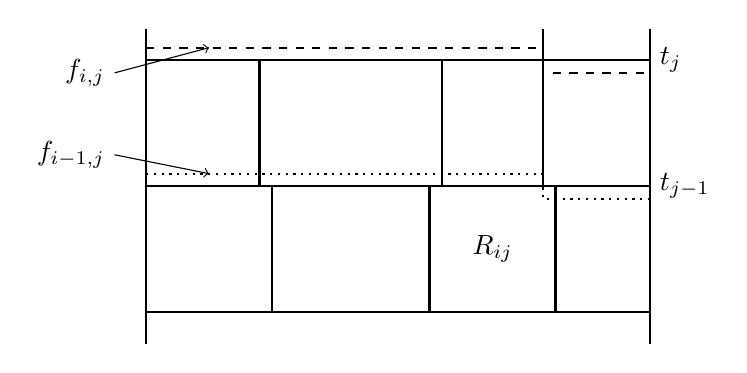
\begin{tikzpicture}[scale=0.8]
    % Grid
    \draw[thick] (0,0) -- (8,0);
    \draw[thick] (0,2) -- (8,2);
    \draw[thick] (0,4) -- (8,4);
    
    % Vertical lines with perturbation
    \draw[thick] (0,-0.5) -- (0,4.5);
    \draw[thick] (8,-0.5) -- (8,4.5);
    \draw[thick] (2,0) -- (2,2); \draw[thick] (1.8,2) -- (1.8,4);
    \draw[thick] (4.5,0) -- (4.5,2); \draw[thick] (4.7,2) -- (4.7,4);
    \draw[thick] (6.5,0) -- (6.5,2); \draw[thick] (6.3,2) -- (6.3,4.5);

    % Labels
    \node at (5.5,1) {$R_{ij}$};
    \node[right] at (8,2) {$t_{j-1}$};
    \node[right] at (8,4) {$t_j$};
    
    % Dotted loops fij
    \draw[thick, dotted] (0,2.2) -- (6.3,2.2) -- (6.3,1.8) -- (8,1.8);
    \draw[thick, dashed] (0,4.2) -- (6.3,4.2) -- (6.3,3.8) -- (8,3.8);
    
    \draw[<-] (1,2.2) -- (-0.5,2.5) node[left] {$f_{i-1,j}$};
    \draw[<-] (1,4.2) -- (-0.5,3.8) node[left] {$f_{i,j}$};
\end{tikzpicture}
\end{center}

The restriction of $F$ to the rectangle $R_{ij}$ gives a homotopy from $f_{i-1,j}$ to $f_{ij}$, and in this way the homotopy $F$ is broken up into a sequence of smaller homotopies:
\[
f \simeq f_{01} \simeq f_{11} \simeq f_{21} \simeq \cdots \simeq f_{m1} \simeq f_{02} \simeq f_{12} \simeq f_{22} \simeq \cdots \simeq f_{mn}
\]
Some of these homotopies, for example $f \simeq f_{01}$ and $f_{m1} \simeq f_{02}$, are just reparametrizations since the left and right edges of $I \times I$ map to the basepoint $x_0$. The final path $f_{mn}$ is the constant loop.

Let us call the corners of the $R_{ij}$'s \textit{vertices}. For each vertex $v$ with $F(v) \neq x_0$, choose a path $g_v$ from $x_0$ to $F(v)$ in the intersection of the two or three $A_{ij}$'s corresponding to the $R_{ij}$'s containing $v$. If we insert into $f_{ij}$ the appropriate paths $\bar{g}_v g_v$ at successive vertices, as in the first paragraph of the proof, then we obtain a product $f_{ij}^1 f_{ij}^2 \cdots$ homotopic to $f_{ij}$, with each $f_{ij}^k$ a loop in a single $A_\alpha$, namely the $A_{pq}$ corresponding to one of the at most two $R_{pq}$'s containing the relevant horizontal or vertical segment. Making a choice of such an $A_\alpha$ for each $f_{ij}^k$ gives a way of writing $[f_{ij}] \in \pi_1(X)$ as $\Phi(w_{ij})$ for a word $w_{ij} = w_{ij}^1 w_{ij}^2 \cdots$ in $*_\alpha \pi_1(A_\alpha)$, with $w_{ij}^k = [f_{ij}^k]$. Making a different choice $A_\beta$ instead of $A_\alpha$ changes the corresponding $w_{ij}^k$ from $w_{ij}^k = i_{\alpha\beta}(\omega) \in \pi_1(A_\alpha)$ to $w_{ij}^k = i_{\beta\alpha}(\omega) \in \pi_1(A_\beta)$. Hence $w_{ij}$ changes from a product of the form $\omega_1 i_{\alpha\beta}(\omega) \omega_2$ to $\omega_1 i_{\beta\alpha}(\omega) \omega_2$. Modulo the normal subgroup $N$, these two $w_{ij}$'s are equivalent since
\[
\omega_1 i_{\alpha\beta}(\omega) \omega_2 = [\omega_1 i_{\alpha\beta}(\omega) i_{\beta\alpha}(\omega)^{-1} \omega_1^{-1}] \omega_1 i_{\beta\alpha}(\omega) \omega_2
\]
and the bracketed expression is in $N$.

The homotopy $f_{i-1,j} \simeq f_{ij}$ across $R_{ij}$ changes the subword of $w_{i-1,j}$ corresponding to the left and bottom edges of $R_{ij}$ to the subword of $w_{ij}$ corresponding to the upper and right edges of $R_{ij}$. If we choose the terms in these subwords to lie in $\pi_1(A_{ij})$, then the homotopy across $R_{ij}$ shows that these two subwords define the same element of $\pi_1(A_{ij})$, hence $w_{i-1,j} = w_{ij}$ in $*_\alpha \pi_1(A_\alpha)$. Thus we have shown that the image of $w_{ij}$ in $*_\alpha \pi_1(A_\alpha)/N$ is independent of $i$ and $j$.

We may assume that the homotopy $F(s,t)$ is independent of $t$ in the bottom row of rectangles $R_{i1}$. Then since the $s_i$-partition subdivides the partition defining the factorization $f = f_1 \cdots f_k$, the bottom edge of each $R_{i1}$ is contained in the domain of an $f_\ell$ and we may choose $A_{i1}$ to be the $A_\alpha$ for which $[f_\ell] \in \pi_1(A_\alpha)$. The effect of this is that the word $w_{01}$ reduces to $w = w_1 \cdots w_k$ in $*_\alpha \pi_1(A_\alpha)$. The final word $w_{mn}$ is the identity element of $*_\alpha \pi_1(A_\alpha)$ since $f_{mn}$ is the constant loop. Applying the conclusion of the preceding paragraph, we deduce that $w$ has trivial image in $*_\alpha \pi_1(A_\alpha)/N$, finishing the proof. 
\end{proof}

\noindent\textbf{Example:}
\begin{itemize}
    \item \textit{Wedge Sum:} $\bigvee_\alpha X_\alpha$ at basepoint $x_\alpha \in X_\alpha$ is $\bigsqcup_\alpha X_\alpha / \{ x_\alpha \sim x_\alpha'\}$. Assume that $\{X_\alpha\}$ path-connected, then $\bigvee_\alpha X_\alpha$ is path-connected. Take $U_\alpha \ni x_\alpha$ to be an open neighborhood defomation retract to $x_\alpha$. Then for any $\alpha$, $A_\alpha := X_\alpha \vee (\bigvee_{\beta \neq \alpha} U_\beta)$ is an open neighborhood of $x_\alpha$ in $\bigvee_\alpha X_\alpha$, deformation retract to $x_\alpha$. Since $A_\alpha \cap A_\beta = \bigvee_\gamma U_\gamma$ deformation retract to point, then $\Pi_1 (A_\alpha \cap A_\beta) =\{e\}$. Hence,
    $$\Pi_1(\bigvee_\alpha X_\alpha) \cong *_\alpha \Pi_1 (A_\alpha) \cong *_\alpha \Pi_1 (X_\alpha)$$

    \item \textit{Finite Graph:} Let $X$ be a path-connected space defined by connected finite graph with $V$ vertices, $E$ edges. Set $g:= 1-V+E$. Then
    $$\Pi_1(X) \cong F_g$$
    \begin{proof}
        Let $T$ be a maximal tree of $X$. Recall that $T$ is contractible and that $T$ contains all the vertices of $X$. Adding a new edge $e_\alpha$ to $T$, then we can get $T \cup \{ e_\alpha\} \simeq \mathbb{S}^1$. Continuing adding edge in $X \setminus T$, then we are done.
    \end{proof}

    \item \textit{Suspension of 3 points:} Let $X$ be the suspension of 3 points, i.e.:
    $$X:= S\{ x,y,z\} := \{x,y,z\} \times I/ (\{x,y,z\} \times \{0\} \cup \{x,y,z\} \times \{1\})$$
    Take $X_\omega$ for $\omega \in \{x,y,z\}$ open cover as $X\setminus \{\omega\}$. Then $X_\omega \cap X_{\omega'}$ is contractible. Hence,
    $$\Pi_1 (X) \cong \Pi_1(X_\omega) * \Pi_1(X_{\omega'}) \cong \mathbb{Z} * \mathbb{Z}$$
\end{itemize}